
\normalsize

\section{Model}

\begin{definition}[Change the Matches of a Predicate-Based Read]
A transaction $T_i$ changes the matches
of a predicate-based read $r_j$(P:Vset(P)) if $T_i$ installs $x_i$, $x_h$
immediately precedes $x_i$ in the version order, and $x_h$ matches
P whereas $x_i$ does not or vice-versa. In this case, we also
say that $x_i$ changes the matches of the predicate-based read.
The above definition identifies $T_i$ to be a transaction where
a change occurs for the matched set of $r_j$ (P: Vset(P)).
\end{definition}

\begin{definition}[Directly Read-Depends]
$T_j$ directly read-depends on transaction $T_i$ if it directly
item-read-depends or directly predicate-read-depends on $T_i$.
\end{definition}

\begin{definition}[Directly item-read-depends by $x$]
$T_j$ directly item-read-depends on transaction $T_i$ if $T_i$ installs some
  object version $x_i$ and $T_j$ reads $x_i$.
\end{definition}

\begin{definition}[Directly item-read-depends]
$T_j$ directly item-read-depends on transaction $T_i$ if $T_j$
  directly item-read-depends by $x$ on $T_i$ for some data item $x$.
\end{definition}

\begin{definition}[Directly predicate-read-depends by $P$]
Transaction $T_j$ directly predicate-read-depends by $P$ on
transaction $T_i$ if $T_j$ performs an operation $r_j$(P: Vset(P)),
$x_k$ $\in$ Vset(P), $i = k$ or $x_i \ll x_k$ , and $x_i$ changes the
matches of $r_j$ (P: Vset(P)).
\end{definition}

\begin{definition}[Directly predicate-read-depends]
$T_j$ directly predicate-read-depends on $T_i$ if $T_j$ directly
  predicate-read-depends by $P$ on $T_i$ for some predicate $P$.
\end{definition}

\begin{definition}[Directly Anti-Depends]
Transaction $T_j$ directly anti-depends on transaction $T_i$ if it
directly item-anti-depends or directly predicate-anti-depends on
$T_i$.
\end{definition}

\begin{definition}[Directly item-anti-depends by $x$]
$T_j$ directly item-anti-depends by $x$ on transaction $T_i$ if $T_i$
  reads some object version $x_k$ and $T_j$ installs $x$'s next
  version (after $x_k$) in the version order. Note that the
  transaction that wrote the later version directly item-anti-depends
  on the transaction that read the earlier version.
\end{definition}

\begin{definition}[Directly item-anti-depends]
$T_j$ directly item-anti-depends on transaction $T_i$ if $T_j$
  directly item-anti-depends on transaction $T_i$.
\end{definition}

\begin{definition}[Directly predicate-anti-depends by $P$]
$T_j$ directly predicate-anti-depends by $P$ on transaction $T_i$ if
  $T_j$ overwrites an operation $r_i(P:$ Vset(P)). That is, if $T_j$
  installs a later version of some object that changes the matches of
  a predicate based read performed by $T_i$.
\end{definition}

\begin{definition}[Directly predicate-anti-depends by $P$]
$T_j$ directly predicate-anti-depends on transaction $T_i$ if $T_j$
  directly predicate anti-depends by $P$ on $T_i$ for some predicate
  $P$.
\end{definition}

\begin{definition}[Directly Write-Depends by $x$]
A transaction $T_j$ directly write-depends by $x$ on transaction $T_i$
if $T_i$ installs a version $x_i$ and $T_j$ installs $x$'s next
version (after $x_i$) in the version order.
\end{definition}

\begin{definition}[Directly Write-Depends]
A transaction $T_j$ directly write-depends on transaction $T_i$ if
$T_i$ directly write-depends by $x$ on $T_j$ for some item $x$.
\end{definition}

\begin{definition}[Directly Session-Depends by $S$]
A transaction $T_j$ directly session-depends on transaction $T_i$ if
$T_i$ immediately precedes $T_j$ in the session commit order for session $S$.
\end{definition}

\begin{definition}[Directly Session-Depends]
A transaction $T_j$ directly session-depends on transaction $T_i$ if
$T_j$ directly session-depends on transaction $T_i$ for some session
$S$.
\end{definition}

\section{HAT Guarantees}

\begin{definition}[Read Uncommitted]
\end{definition}

\begin{definition}[Read Committed]
\end{definition}

\begin{definition}[Item Cut Non-Isolation (N-ICI)]
A history $H$ exhibits phenomenon N-ICI if there exists a transaction
$T_i$ such that $T_i$ directly item-depends by $x$ on more than one
other transaction.
\end{definition}

\begin{figure}[H]
\begin{align*}
\small
T_1 &: w_x(1)\\
T_2 &: w_x(2)\\
T_3 &: r_x(1)~r_x(2)
\end{align*}
\caption{Example of \textit{N-ICI} anomaly.}
\label{fig:nici-history}
\end{figure}

\begin{figure}[H]
\centering
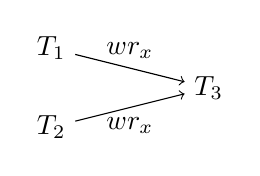
\begin{tikzpicture}[node distance=3cm]
\tikzstyle{tx}=[draw=none, fill=none]
\node[tx] (T1) at (0,0) {$T_1$};
\node[tx] (T2) at (0,-1) {$T_2$};
\node[tx] (T3) at (2,-.5) {$T_3$};

\draw[->] (T1) edge node[above]{$wr_x$} (T3);
\draw[->] (T2) edge node[below]{$wr_x$} (T3);
\end{tikzpicture}
\caption{DSG for Figure~\ref{fig:nici-history}.}
\label{fig:nici-dsg}
\end{figure}

\begin{definition}[Item Cut Isolation (ICI)]
A system that provides Item Cut Isolation prohibits phenomenon N-ICI.
\end{definition}

\begin{definition}[Predicate Cut Non-Isolation (N-ICI)]
A history $H$ exhibits phenomenon N-ICI if there exists a transaction
$T_i$ such that $P= \{p \mid T_i$ directly predicate-read-depends by
$p$ on another other transaction$\}$ and $\bigcap_{p\in P} P \neq
\emptyset$. (TODO: this isn't necessarily it)
\end{definition}

\begin{definition}[Predicate Cut Isolation (ICI)]
A system that provides Predicate Cut Isolation prohibits phenomenon N-ICI.
\end{definition}

\begin{definition}[Non-transactional Atomicity (N-TA)]
A history exhibits phenomenon N-TA if it contains a directed cycle
consisting of exactly one read-dependency edge by $x$ from $T_i$ to
$T_j$ and one anti-dependency edge by $y$ from $T_j$ to $T_i$ and
$T_i$'s corresponding read from $x$ does not precede its corresponding
read from $y$.
\end{definition}


\begin{figure}[H]
\begin{align*}
\small
T_1 &: w_x(1)~w_y(1)\\
T_2 &: w_x(2)~w_y(2)\\
T_3 &: r_x(2)~r_y(1)
\end{align*}
\caption{Example of \textit{N-TA} anomaly.}
\label{fig:nta-history}
\end{figure}

\begin{figure}[H]
\centering
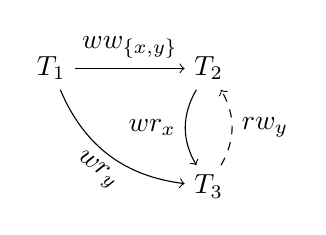
\begin{tikzpicture}[node distance=3cm]
\tikzstyle{tx}=[draw=none, fill=none]
\node[tx] (T1) at (0,0) {$T_1$};
\node[tx] (T2) at (2,0) {$T_2$};
\node[tx] (T3) at (2,-1.5) {$T_3$};

\draw[->] (T1) edge node[sloped, above]{$ww_{\{x, y\}}$} (T2);
\draw[->] (T1) edge [bend right] node[sloped, below]{$wr_y$} (T3);
\draw[->] (T2) edge [bend right] node[left]{$wr_x$} (T3);
\draw[dashed, ->] (T3) edge [bend right] node[right]{$rw_y$} (T2);
\end{tikzpicture}
\caption{DSG for Figure~\ref{fig:nta-history}.}
\label{fig:nta-dsg}
\end{figure}

\begin{definition}[Transactional Atomicity (TA)]
A system that provides transactional atomicity prohibits phenomenon
N-TA.
\end{definition}

\begin{definition}[Non-monotonic Reads (N-MR)]
A history exhibits phenomenon N-MR if it contains a directed cycle
consisting of a transitive session-dependency between transactions
$T_j$ and $T_i$ with an anti-dependency edge by $i$ from $T_j$ and a
read-dependency edge by $i$ into $T_i$.
\end{definition}

\begin{definition}[Monotonic Reads (MR)]
A system provides Monotonic Reads if it prohibits phenomenon N-MR.
\end{definition}


\begin{figure}[H]
\begin{align*}
\small
T_1 &: w_x(1)\\
T_2 &: w_x(2)\\
T_3 &: r_x(2)\\
T_4 &: r_x(1)
\end{align*}
\caption{Example of \textit{N-MR} violation when $w_x(1) \ll w_x(2)$ and $T_4$ directly session-depends on $T_3$.}
\label{fig:nmr-history}
\end{figure}

\begin{figure}[H]
\centering
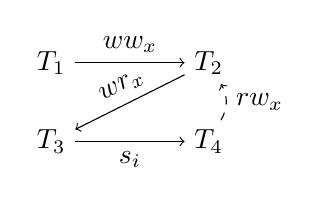
\begin{tikzpicture}[node distance=3cm]
\tikzstyle{tx}=[draw=none, fill=none]
\node[tx] (T1) at (0,0) {$T_1$};
\node[tx] (T2) at (2,0) {$T_2$};

\node[tx] (T3) at (0,-1) {$T_3$};
\node[tx] (T4) at (2,-1) {$T_4$};

\draw[->] (T1) edge node[above]{$ww_x$} (T2);
\draw[->] (T3) edge node[below]{$s_i$} (T4);

\draw[->] (T2) edge node[sloped, above]{$wr_x$} (T3);
%\draw[->] (T2) edge [bend right] node[left]{$wr_x$} (T4);
%\draw[->] (T1) edge [bend right]node[right]{$wr_x$} (T4);
\draw[dashed, ->] (T4) edge [bend right]node[right]{$rw_x$} (T2);
\end{tikzpicture}
\caption{DSG for Figure~\ref{fig:nmr-history}. $wr_x$ dependency from $T_1$ to $T_4$ omitted.} 
\label{fig:nmr-dsg}
\end{figure}

\begin{definition}[Non-monotonic Writes (N-MW)]
A history exhibits phenomenon N-MW if it contains a directed cycle
consisting of a transitive session-dependency between transactions
$T_j$ and $T_i$ and at least one write-dependency edge.
\end{definition}


\begin{figure}[H]
\begin{align*}
\small
T_1 &: w_x(1)\\
T_2 &: w_y(1)\\
T_3 &: r_y(1)~r_x(0)
\end{align*}
\caption{Example of \textit{N-MW} anomaly if $T_2$ directly session-depends on $T_1$.}
\label{fig:nmw-history}
\end{figure}

\begin{figure}[H]
\centering
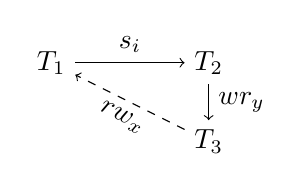
\begin{tikzpicture}[node distance=3cm]
\tikzstyle{tx}=[draw=none, fill=none]
\node[tx] (T1) at (0,0) {$T_1$};
\node[tx] (T2) at (2,0) {$T_2$};
\node[tx] (T3) at (2,-1) {$T_3$};

\draw[->] (T1) edge node[above]{$s_i$} (T2);
\draw[->] (T2) edge node[right]{$wr_y$} (T3);
\draw[->, dashed] (T3) edge node[below, sloped]{$rw_x$} (T1);
\end{tikzpicture}
\caption{DSG for Figure~\ref{fig:nmw-history}.}
\label{fig:nmw-dsg}
\end{figure}


\begin{definition}[Monotonic Writes (MW)]
A system provides Monotonic Writes if it prohibits phenomenon N-MW.
\end{definition}

\begin{definition}[Writes Do Not Follow Reads (N-WFR)]
A history exhibits phenomenon N-WFR if, for all committed transactions
$T_1$, $T_2$, $T_3$ such that $T_2$ write-depends on $T_1$ and $T_3$
write-depends on $T_2$, $T_3$ does not directly anti-depend on $T_1$.
\end{definition}


\begin{figure}[H]
\begin{align*}
\small
T_1 &: w_x(1)\\
T_2 &: r_x(1) w_y(1)\\
T_3 &: r_y(1)~r_x(0)
\end{align*}
\caption{Example of \textit{N-WFR} anomaly.}
\label{fig:nwfr-history}
\end{figure}

\begin{figure}[H]
\centering
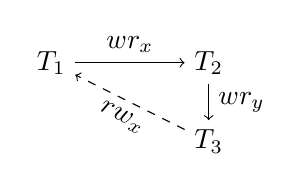
\begin{tikzpicture}[node distance=3cm]
\tikzstyle{tx}=[draw=none, fill=none]
\node[tx] (T1) at (0,0) {$T_1$};
\node[tx] (T2) at (2,0) {$T_2$};
\node[tx] (T3) at (2,-1) {$T_3$};

\draw[->] (T1) edge node[above]{$wr_x$} (T2);
\draw[->] (T2) edge node[right]{$wr_y$} (T3);
\draw[->, dashed] (T3) edge node[below, sloped]{$rw_x$} (T1);
\end{tikzpicture}
\caption{DSG for Figure~\ref{fig:nwfr-history}.}
\label{fig:nwfr-dsg}
\end{figure}

\begin{definition}[Writes Follow Reads (WFR)]
A system provides Writes Follow Reads if it prohibits phenomenon N-WFR.
\end{definition}

\begin{definition}[Not-Read Your Writes (N-RYW)]
A history exhibits phenomenon N-RYW if it contains a directed cycle
consisting of a transitive session-dependency between transactions
$T_j$ and $T_i$, at least one anti-dependency edge, and the remainder
anti-dependency or write-dependency edges.
\end{definition}


\begin{figure}[H]
\begin{align*}
\small
T_1 &: w_x(1)\\
T_2 &: r_x(0)\\
\end{align*}
\caption{Example of \textit{N-RYW} anomaly if $T_2$ directly session-depends on $T_1$.}
\label{fig:nryw-history}
\end{figure}

\begin{figure}[H]
\centering
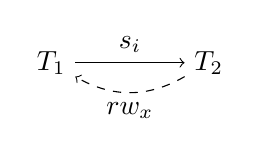
\begin{tikzpicture}[node distance=3cm]
\tikzstyle{tx}=[draw=none, fill=none]
\node[tx] (T1) at (0,0) {$T_1$};
\node[tx] (T2) at (2,0) {$T_2$};

\draw[->] (T1) edge node[above]{$s_i$} (T2);
\draw[dashed, ->] (T2) edge [bend left] node[below]{$rw_x$} (T1);
\end{tikzpicture}
\caption{DSG for Figure~\ref{fig:nwfr-history}.}
\label{fig:nryw-dsg}
\end{figure}

\begin{definition}[Read Your Writes (RYW)]
A system provides Read Your Writes if it prohibits phenomenon N-RYW.
\end{definition}

\begin{definition}[PRAM Consistency]
A system provides PRAM Consistency if it prohibits phenomenon N-MR,
N-MW, and N-RYW.
\end{definition}

\begin{definition}[Causal Consistency]
A system provides Causal Consistency if it provides PRAM Consistency
and prohibits phenomenon N-WFR.
\end{definition}


\begin{observation}
Read Your Writes is not highly available.
\end{observation}

\begin{corollary}
PRAM and Causal Consistency are not highly available.
\end{corollary}

\begin{definition}[Recency Guarantees]
\end{definition}

\begin{definition}[Lost Update]
\end{definition}

\begin{definition}[Write Skew]
\end{definition}

\begin{definition}[Snapshot Isolation]
\end{definition}

\begin{definition}[Repeatable Read]
\end{definition}

\begin{definition}[Safe Register]
\end{definition}

\begin{definition}[Regular Register]
\end{definition}

\begin{definition}[Linearizable Register]
\end{definition}

\begin{definition}[Strong One-copy Serializability]
\end{definition}

\begin{definition}[Model Strength]
We say that a consistency model $M_1$ is stronger than model $M_2$ if
$M_1$ admits a strict subset of the histories admitted by $M_2$.
\end{definition}

\begin{observation}
Transactional Atomicity is weaker than Repeatable Read.
\end{observation}

\begin{observation}
Transactional Atomicity is weaker than Snapshot Isolation.
\end{observation}

\begin{observation}
Causality is weaker than linearizability.
\end{observation}

\begin{observation}
Read Your Writes is weaker than safe register semantics.
\end{observation}

